%license:BSD-3-Clause
%copyright-holders:Michele Maione
%============================================================
%
%	Piattaforma di cloud gaming per giochi arcade
%
%============================================================

\chapter{Architettura del sistema}
%In questa sezione si deve descrivere l’obiettivo della ricerca, le problematiche affrontate ed eventuali definizioni preliminari nel caso la tesi sia di carattere teorico.
In questo capitolo verrà descritto il sistema proposto, il MAME e le sue funzioni di: rendering, missaggio audio e gestione dell'input utente.



\section{Sistema proposto}
L'esigenza per la quale nasce questo progetto è far conoscere alle nuove generazioni i videogiochi che hanno fatto la storia e dare la possibilità di poter giocare ancora a macchine che ormai hanno cessato di funzionare per motivi di obsolescenza, sfruttando due tecnologie entrate a far parte della quotidianità, lo streaming e il cloud computing. In questo lavoro si propone la creazione di una piattaforma di cloud gaming, che permette lo streaming audio-video direttamente e su richiesta dei videogiochi, da un server remoto, ad un client (computer, console, telefono). Per far ciò verrà ampliato il software MAME (rilasciato sotto licenza GNU-GPL) che è in grado di emulare oltre 7.000 giochi arcade. Le caratteristiche principali del progetto, che sono state vincolanti nella scelta delle tecnologie da utilizzare, sono la portabilità e la possibilità di utilizzare il sistema senza dover installare software aggiuntivi, e per questi vincoli, lato client, la scelta è ricaduta sul browser web.

Il sistema è stato progettato con un'ottica incentrata sull'utilizzo in LAN con l'utenza connessa tramite WiFi, ad esempio in stand di retro-gaming ad eventi di informatica e videogiochi, in aziende come servizio di svago per i clienti in sala d'attesa e per i dipendenti durante la pausa, ecc\dots, è importante ricordare che i videogiochi, nonostante siano stati pensati come fonte d'intrattenimento, migliorano diversi tipi di abilità chiave: abilità sociali e intellettuali, riflessi e concentrazione \parencite{Use_of_Cloud_Gaming_in_Education}; per questo motivo la piattaforma può essere installata anche nelle scuole. La tecnologia di streaming scelta è stata WebSocket per i seguenti motivi: in questo contesto la differenza di velocità tra TCP e RTP può essere trascurata, è un protocollo di comunicazione standardizzato dal 2011, è pienamente supportato da tutti i browser moderni, ha una latenza inferiore rispetto ad HLS e DASH, è semplice da instanziare e non richiede l'utilizzo di protocolli aggiuntivi o configurazioni complesse a differenza di WebRTC.

Come mostrato in Fig. \ref{fig:proposed_system} il sistema è costituito dal server di gioco (Linux, Windows o macOS), su cui è installato il MAME CGP con le rom dei giochi ed una pagina HTML5 che funge da front-end. Il programma è in ascolto per connessioni WebSocket con parametri (per es.: il nome del gioco, l'ID del player, l'ID della partita, ecc\dots). Una volta stabilita la connessione, il server invia informazioni sulla risoluzione di rendering e avvia il gioco. Il rendering e il missaggio audio del gioco vengono generati utilizzando la libreria SDL, codificati e pacchettizzati nel contenitore MPEG-TS\footnote{MPEG-TS: MPEG transport stream, è un contenitore digitale per la trasmissione e l'archiviazione audio-video.} usando la libreria FFmpeg\footnote{FFmpeg è una suite open-source di librerie e programmi per la gestione di video, audio, e altri file multimediali e stream.} e inviati tramite WebSocket al client.

\begin{figure}[H]
	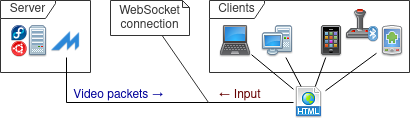
\includegraphics[width=\linewidth]{immagini/proposed_system}
	\caption{Panoramica del sistema}
	\label{fig:proposed_system}
\end{figure}

Lato client vari script si occupano di: decodificare i dati audio-video ricevuti, catturare e inviare l'input dell'utente (sia dalla tastiera che dal gamepad) al server tramite WebSocket.

Nel prossima sezione introdurremo il software MAME su cui si basa questo progetto.

\section{MAME}
Multiple Arcade Machine Emulator (MAME) è un progetto open-source (GNU-GPL) di Nicola Salmoria. La prima versione del MAME risale al febbraio 1997 ed è attualmente supportato da una vasta comunità di sviluppatori da tutto il mondo. Lo scopo principale è quello di essere un riferimento al funzionamento interno delle macchine emulate, sia per scopi educativi che per scopi di conservazione, al fine di evitare che il software storico scompaia per motivi di obsolescenza. Il progetto è stato realizzato in C++, inizialmente usando solamente la libreria standard e poi successivamente, negli anni, sono state aggiunte al progetto varie librerie open-source per estenderne le funzionalità. Originariamente era disponibile solo per MS-DOS ma grazie alla vasta comunità di sviluppatori è stato portato per i sistemi Windows e Unix-like \parencite{MAME}. Logicalmente è suddiviso in quattro macro categorie, come mostrato in Fig. \ref{fig:mame_arch}:

\begin{figure}[H]
	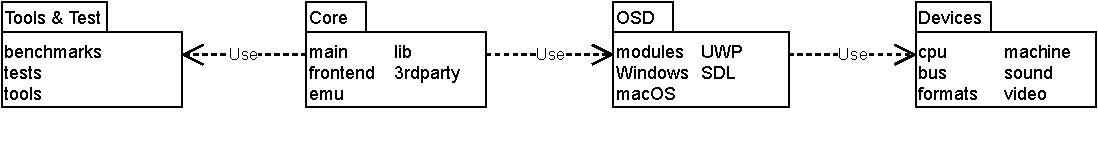
\includegraphics[width=\linewidth]{immagini/mame_arch}
	\caption{MAME, diagramma dei packages}
	\label{fig:mame_arch}
\end{figure}

\begin{itemize}
	\item "Core" in cui ci sono i sotto-progetti indipendenti dal sistema e dal device emulato tra cui il programma principale (progetto main), il front-end grafico, il motore di emulazione (progetto emu), le librerie comuni (lib) ed i sorgenti delle librerie esterne (3rdparty);
	\item "OSD" contenente le funzionalità sia dipendenti dal sistema operativo come macOS, Windows, UWP ed SDLMAME, sia i moduli (progetto modules) di input, audio e video dipendenti da altre librerie come OpenGL, DirectX, SDL, CoreAudio, XAudio, XInput, ecc\dots;
	\item "Devices" che contiene per ogni device emulato (ad esempio il Capcom CP System III) le classi che gestiscono le informazioni della macchina ed emulano cpu, bus, video, audio e i dischi (progetto formats);
	\item "Tools \& Test" che contiene varie utility per la gestione delle rom e per la fase di testing.
\end{itemize}

\textit{Il progetto ha una struttura modulare}, schematizzata in Fig. \ref{fig:mame_schema_moduli_d}, \textit{formato da un nucleo centrale che dirige le operazioni, gestisce l’interfaccia utente e mette a disposizione dei driver un buon numero di funzioni d'uso comune. Il nucleo delega a moduli esterni l'emulazione dei vari tipi di CPU e di chip audio supportati. In pratica il nucleo fornisce un ambiente operativo specializzato nell'emulazione di videogiochi arcade, che i driver possono sfruttare con poco codice aggiuntivo. Spesso la maggior parte del contenuto di un driver è costituita da strutture dati, gestite direttamente dal nucleo. Il driver deve fornire codice solo per alcuni compiti specifici, ad esempio l'aggiornamento del video} \parencite{Il_progetto_MAME}.

\begin{figure}[H]
	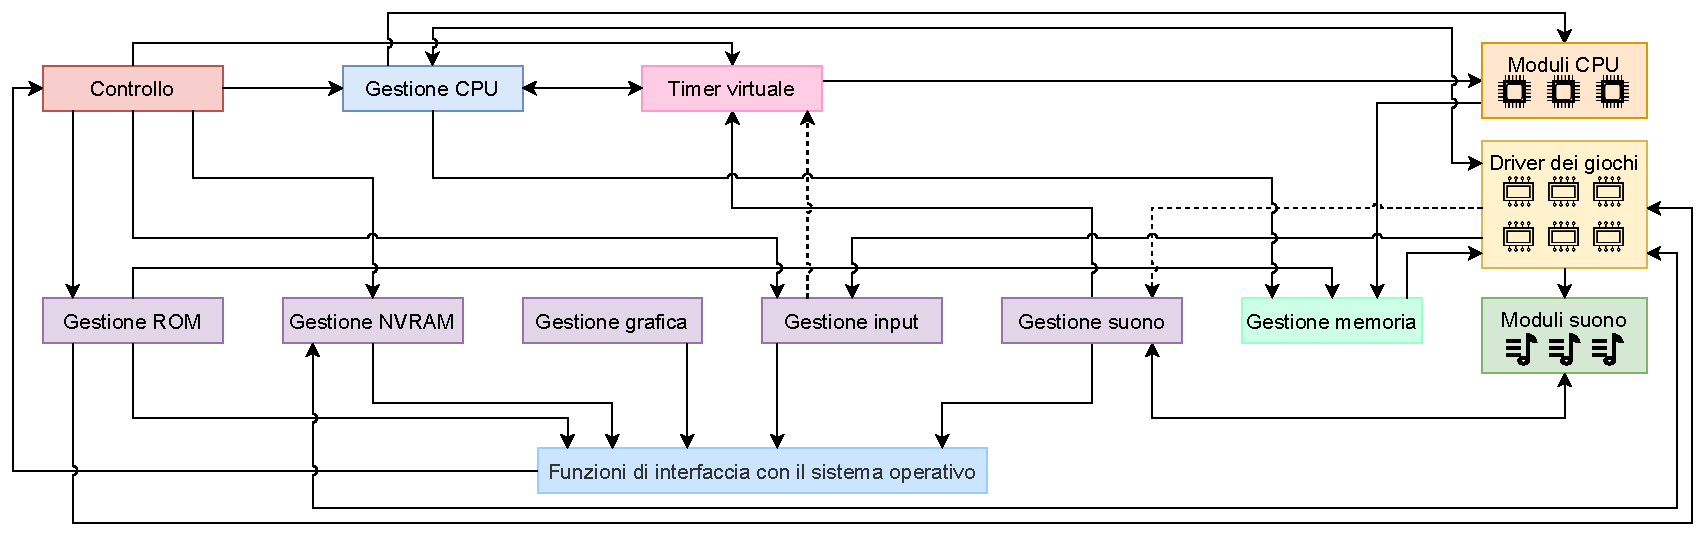
\includegraphics[width=\linewidth]{immagini/mame_schema_moduli_d}
	\caption{Schema della struttura di MAME}
	\label{fig:mame_schema_moduli_d}
\end{figure}

Per quanto riguarda la portabilità, di cui c'è uno schema in Fig. \ref{fig:mame_architettura_full}, ci sono solo tre compilazioni native differenti e sono quella per macOS, Windows ed UWP\footnote{UWP: Universal Windows Platform è un'architettura applicativa della Microsoft per sviluppare applicazioni eseguibili su Windows 10, Xbox One e Hololens.}, in aggiunta c'è la compilazione SDLMAME\footnote{SDLMAME era un port del MAME che utilizzava solamente la libreria SDL. Nel 2010 è stato incluso ufficialmente nel progetto MAME.} in grado di funzionare su tutti i sistemi operativi supportati dalla libreria SDL. Quest'ultima è la compilazione obbligatoria per i sistemi Linux e per questo motivo è quella che si è scelta di utilizzare per questo server di cloud gaming.

\begin{figure}[H]
	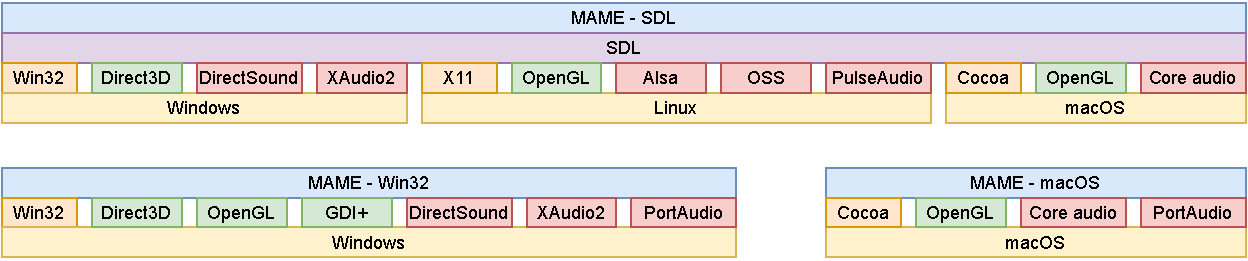
\includegraphics[width=\linewidth]{immagini/mame_architettura_full}
	\caption{Librerie e interfacce utilizzate dal MAME sulle diverse piattaforme}
	\label{fig:mame_architettura_full}
\end{figure}

SDL (Simple DirectMedia Layer) è una libreria multipiattaforma che fornisce accesso di basso livello ad audio, tastiera, mouse, gamepad, hardware 3D e framebuffer 2D. Come mostrato in Fig. \ref{fig:mame_architettura_full} nello schema in alto, SDL è costruito sopra le API di visualizzazione video del sistema operativo (in arancione), le librerie di rendering 3D (in verde) e le librerie che si interfacciano alla scheda audio (in rosso) \parencite{SDL_Wiki}.

Nel prossimi tre paragrafi verrano descritti i tre moduli su cui sono state apportate delle modifiche per trasformare il MAME in una piattaforma di cloud gaming.


\subsection{Rendering}
Il rendering è il processo di generazione di un'immagine a partire dalla sua descrizione, che può essere sia in due dimensioni (2D) sia in tre (3D), tramite un software. Gli elementi di base del rendering 2D sono le textures\footnote{Una texture è un'immagine rappresentata come una matrice bidimensionale di pixel colorati (in inglese bitmap). Ogni pixel è rappresentato tramite una quaterna formata dai tre colori primari più un valore che ne indica la trasparenza (RGB + A); servono 4 bit per memorizzare ogni elemento della quaterna, quindi 32 in totale per un singolo pixel.} e le animazioni. Il motore grafico (il software che si occupa anche del rendering) prende gli elementi uno ad uno e li disegna nel framebuffer\footnote{Il framebuffer è uno spazio di memoria presente sulla scheda video in cui si memorizza l'immagine che verrà successivamente mostrata a video.} generando l'immagine finale \parencite{Efficient_2D_software_rendering}. Come mostrato in Fig. \ref{fig:rendering_pipeline}, questo processo è formato da quattro fasi \parencite{Computer_Vision_A_Modern_Approach}:

\begin{enumerate}
    \item Trasformazione di modellazione: tramite una trasformazione trasporta le primitive geometriche in un sistema di coordinate universali (\textit{world coordinate system});
    \item Clipping: ritaglia porzioni delle primitive al di fuori della finestra di visualizzazione;
    \item Trasformazione di vista: tramite una trasformazione ridiga detta "trasformazione di vista" trasporta le primiteve ritagliate dalle cordinate universali a quelle schermo (\textit{screen coordinate});
    \item \textit{Scan conversion}: attraverso algoritmi di rasterizzazione\footnote{La rasterizzazione è il processo di approssimazione delle primitive geometriche in immagini bitmap.} genera l'immagine finale.
\end{enumerate}

\begin{figure}[H]
	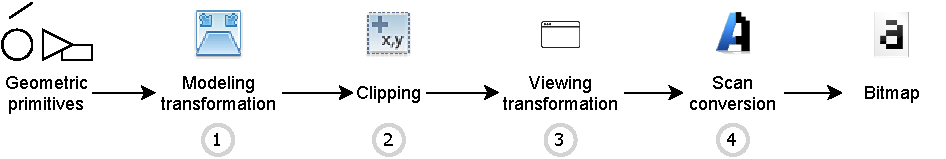
\includegraphics[width=\linewidth]{immagini/rendering_pipeline}
	\caption{Pipeline di rendering 2D}
	\label{fig:rendering_pipeline}
\end{figure}

Il MAME è in grado di emulare giochi sia 2D che 3D (es.: Tekken della Namco) ma sia per la volontà di emulare fedelmente l'hardware della macchina sia perché le varie schede ed API grafiche delle macchine emulate non lavorano esattamente come quelle moderne (es.: i poligoni della mesh utilizzano i rettangoli al posto dei triangoli) tutta la fase di rendering viene eseguita via software, per questo motivo ciò che viene inviato alla libreria grafica è un insieme di primitive e texture da disegnare sia nel caso di giochi 2D che 3D come spiegato nella FAQ ufficiale nel capitolo sulle performance: \textit{«There are many things that are difficult to emulate without expending a large amount of CPU power. Some specific examples are: Games with 3D graphics. As of this writing, MAME does not pass polygons down to the video card of your system; instead, it renders all 3D graphics by hand in software. Although this code is generally optimized to take advantage of multiple CPUs, it is still quite taxing to do this. Some 3D games give you control of the output resolution; reducing it will reduce the CPU requirements.»} \parencite{MAME_FAQ_Performance}.

È importante sottolineare che l'interfaccia grafica del MAME viene disegnata con le stesse procedure utilizzate per l'emulazione, e questo consente al nostro progetto di poter effettuare lo streaming anche dell'interfaccia grafica che può essere usata al posto del front-end HTML.

\begin{figure}[H]
	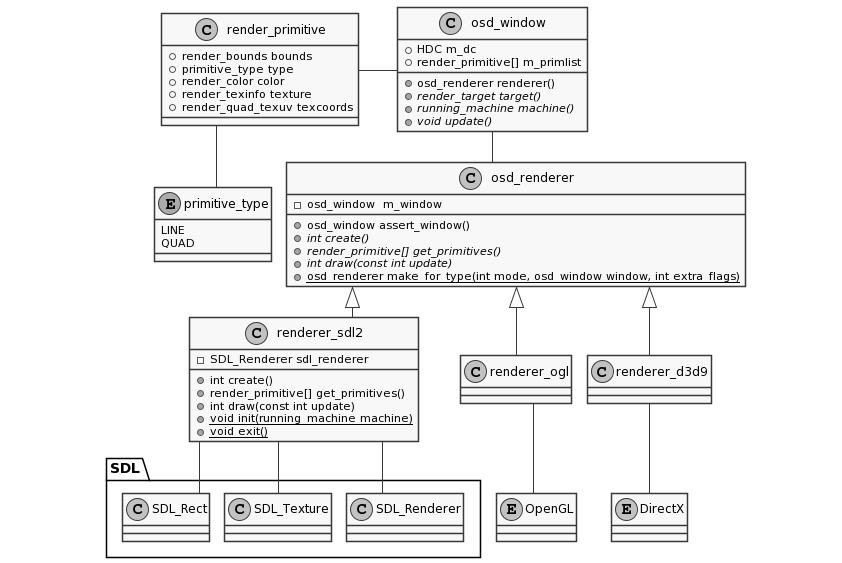
\includegraphics[width=\linewidth]{immagini/class_renderingSDLFull}
	\caption{Diagramma delle classi relative al rendering}
	\label{fig:class_renderingSDLFull}
\end{figure}

Come detto precedentemente il MAME supporta varie librerie multimediali per la fase di rendering e di missaggio audio. In Fig. \ref{fig:mame_render_class_diagram} è visibile un diagramma delle classi relativo alla sola funzionalità di rendering da cui è stato estrapolato il diagramma parziale di Fig. \ref{fig:class_renderingSDLFull}. Dopo che è stata creata la finestra in cui verrà visualizzato il rendering, tramite la funzione \verb|osd_renderer::make_for_type| viene istanziata una delle classi per il rendering (es.: \verb|render_ogl|, \verb|render_d3d9|, \verb|renderer_sdl2|, ecc\dots) che comunica direttamente con la libreria grafica. Alla creazione di una di queste classi viene chiamato il metodo \verb|osd_renderer::create| che si occupa di inizializzare il necessario per il rendering. Per ogni frame della macchina che viene emulato c'è una fase di disegno tramite il metodo \verb|osd_renderer::draw|.

La classe che si occupa del rendering utilizzando la libreria SDL è \verb|renderer_sdl2| che utilizza le seguenti funzioni SDL:

\begin{itemize}	
	\item \verb|SDL_CreateRenderer|: Crea un contesto di rendering 2D per una finestra;
	\item \verb|SDL_SetRenderDrawColor|: Imposta il colore utilizzato per le operazioni di disegno;
	\item \verb|SDL_RenderFillRect|: Riempe un rettangolo con il colore di disegno corrente; è usato per disegnare la primitiva \verb|QUAD|;
	\item \verb|SDL_RenderDrawLine|: Disegna una linea con il colore di disegno corrente; è usato per disegnare la primitiva \verb|LINE|;
	\item \verb|SDL_RenderPresent|: Aggiorna il contesto di rendering con il framebuffer corrente.
\end{itemize}

Di cui la prima viene utilizzata durante la fase di inizializzazione nella funzione \verb|create|, mentre le altre vengono utilizzate durante la fase di disegno nella funzione \verb|draw|.

\subsection{Missaggio audio}

Il missaggio audio è quel procedimento con cui due o più campioni audio sono fusi in un unico output sonoro. La classe che si occupa del missaggio audio utilizzando la libreria SDL è \verb|sound_sdl2| che utilizza le seguenti funzioni SDL:

\begin{itemize}	
	\item \verb|SDL_OpenAudio|: Apre il dispositivo audio;
	\item \verb|SDL_PauseAudio|: Mette in pausa o ripristina la riproduzione audio;
	\item \verb|SDL_CloseAudio|: Interrompere l'elaborazione audio e chiude il dispositivo audio.
\end{itemize}

La funzione \verb|SDL_OpenAudio| utilizza la struttura \verb|SDL_AudioSpec| che contiene informazioni come il formato del buffer audio, il numero di canali, i bit per canale, ecc\dots, e un puntatore ad una funzione di callback; questa funzione è molto importante perché è quella che effettivamente viene utilizzata per riprodurre un suono. Come è visibile in Fig. \ref{fig:class_mixingSDLFull} la funzione \verb|sdl_callback| ha due parametri \verb|stream| e \verb|len| che sono rispettivamente il buffer da riempire con il suono e la dimensione del buffer \parencite{FocusOnSDL}. 

\begin{figure}[H]
	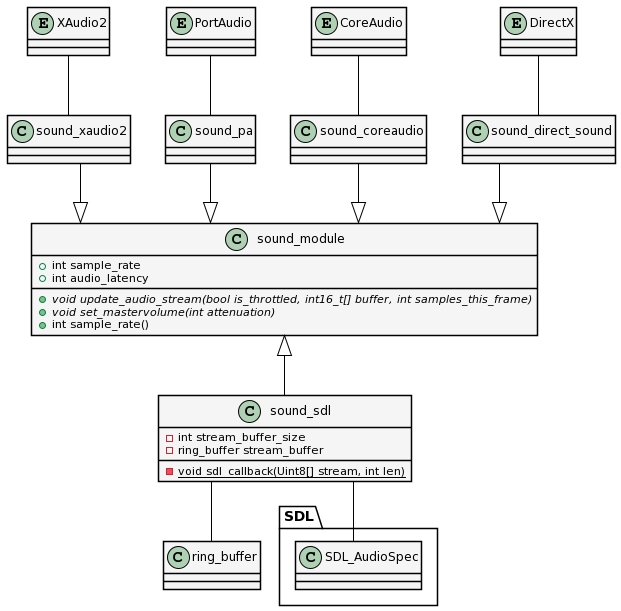
\includegraphics[width=\linewidth]{immagini/class_mixingSDLFull}
	\caption{Diagramma delle classi relative al missaggio audio}
	\label{fig:class_mixingSDLFull}
\end{figure}

\subsection{Gestione input}
Lorem ipsum dolor sit amet, consectetur adipiscing elit, sed do eiusmod tempor incididunt ut labore et dolore magna aliqua. Ut enim ad minim veniam, quis nostrud exercitation ullamco laboris nisi ut aliquip ex ea commodo consequat. Duis aute irure dolor in reprehenderit in voluptate velit esse cillum dolore eu fugiat nulla pariatur. Excepteur sint occaecat cupidatat non proident, sunt in culpa qui officia deserunt mollit anim id est laborum \parencite{SDL_game_development}.

\parencite{CPP_Primer}
\parencite{Computer_Networking_and_the_Internet}
\parencite{Ingegneria_del_software}
\parencite{Understanding_the_Linux_Kernel}
\parencite{Windows_Server_2012}